\chapter{Dziedzina problemu}

\begin{wrapfigure}{R}{3in}
%%%%%%%%%%%%%%%%%%%%%%%%%%%%%%%%%%%%%%%%%%%%%%%%%%%%%%%%%%%%%%%%%%%%%%%%%%%%%%%%%%%%%%%
%%% You will need to add \usepackage{wrapfig} to your preamble to use textwrapping %%%
%%%%%%%%%%%%%%%%%%%%%%%%%%%%%%%%%%%%%%%%%%%%%%%%%%%%%%%%%%%%%%%%%%%%%%%%%%%%%%%%%%%%%%%
 \centering
 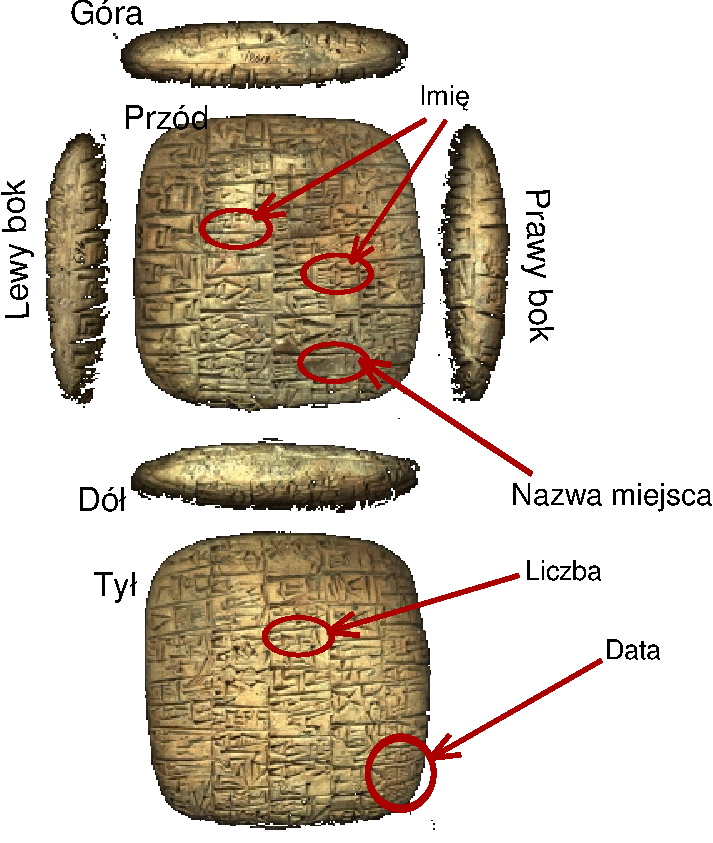
\includegraphics[width=150px]{../diagramy/tabliczka.pdf}
 % tabliczka.pdf: 342x405 pixel, 72dpi, 12.06x14.29 cm, bb=0 0 342 405
 \caption{Gliniana tabliczka - struktura}
\end{wrapfigure}


% \begin{figure}[h]
%  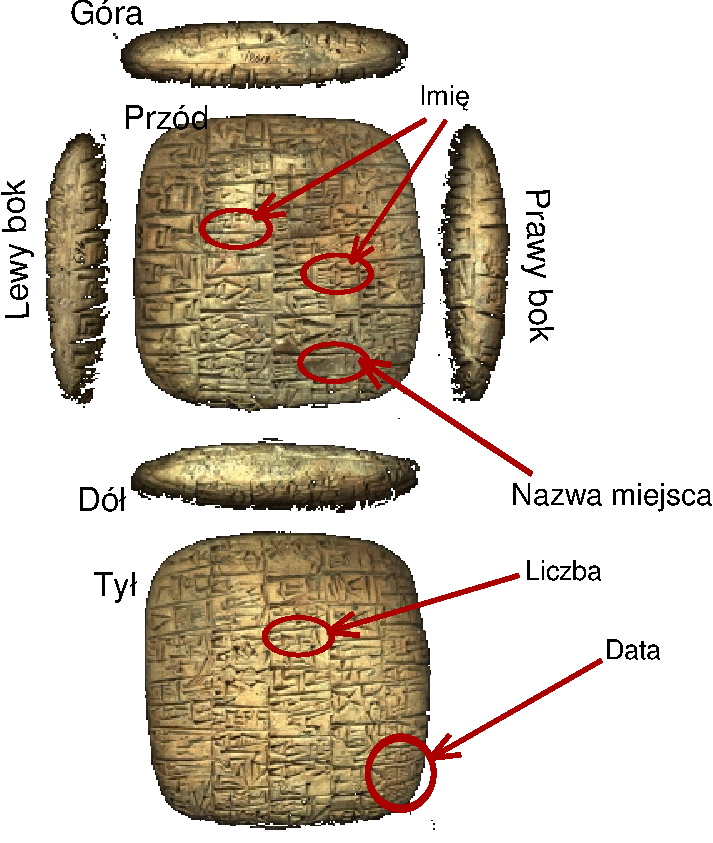
\includegraphics[width=150px]{../diagramy/tabliczka.pdf}
%  % tabliczka.pdf: 342x405 pixel, 72dpi, 12.06x14.29 cm, bb=0 0 342 405
%  \caption{Gliniana tabliczka - struktura}
% \end{figure}

\begin{figure}
 \centering
 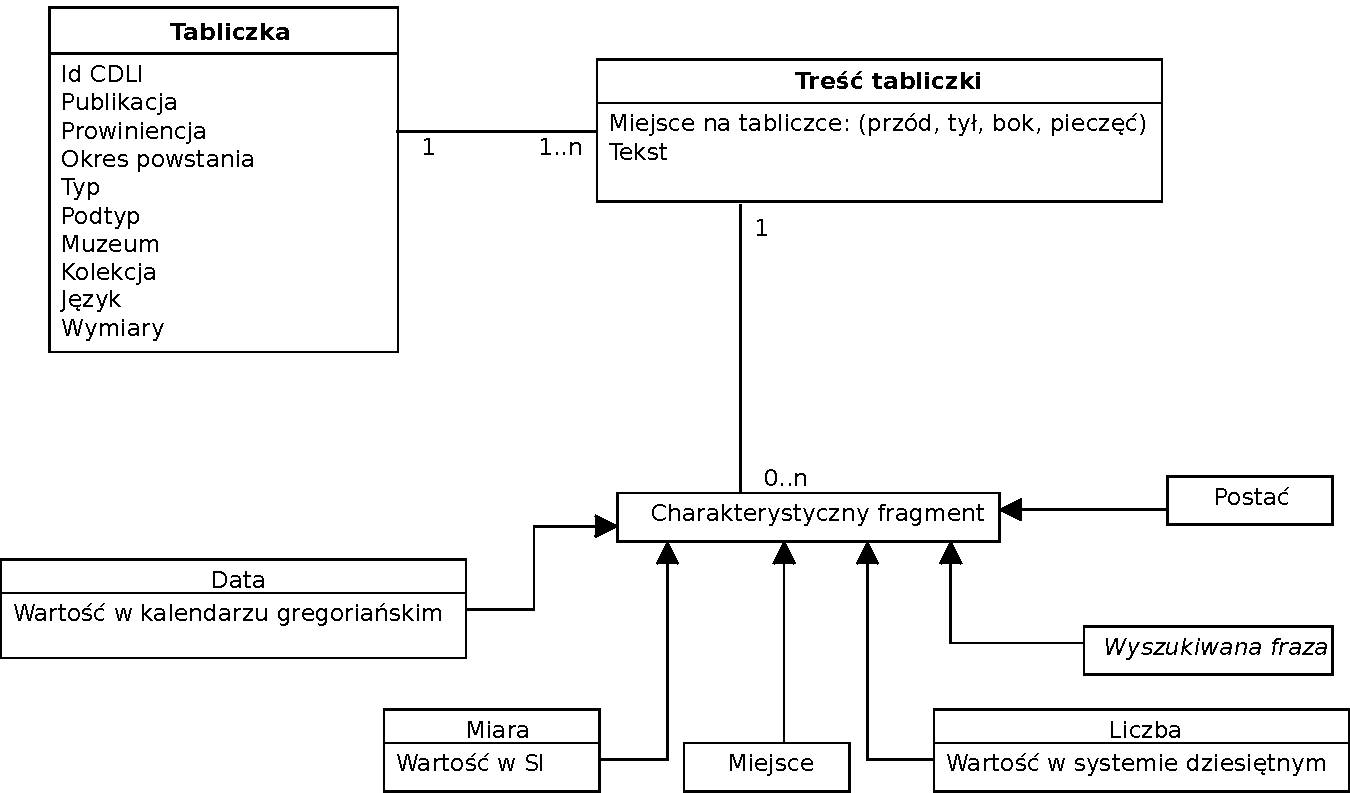
\includegraphics[width=400px]{../diagramy/Model-dziedziny.pdf}
 % Model-dziedziny.png: 650x345 pixel, 72dpi, 22.93x12.17 cm, bb=0 0 650 345
 \caption{Co powinna zawierać tabliczka w formie elektronicznej}
\end{figure}
~ 

Głównym elementem rozpatrywanej przez nas dziedziny jest tabliczka sumeryjska rozumiana dwojako - jako fizyczna tabliczka gliniana oraz jako tabliczka w formie cyfrowej.

Tabliczki gliniane mają różne kształty i wielkość, mogą być zapisane z kilku stron (z przodu, z tyłu, od góry, z boku, itp.) i mogą zawierać pieczęcie, na których również znajduje się tekst. Często są zniszczone lub częściowo uszkodzone. Tekst jest zapisany za pomocą klinów.
Może on zawierać imiona osób i bóstw, liczby, jednostki (np. talent - jednostka wagi), %TODO: sprawdzić
miejsca, daty. Niektóre z tych elementów można przetłumaczyć na współczesny język, na przykład jednostki można przeliczyć na SI, datę opisową na datę wg obecnego kalendarza gregoriańskiego. 

Dla ułatwienia pracy sumerolodzy tłumaczą zapis klinowy na tzw. odczyty, które są sposobem zapisania tekstu sumeryjskiego za pomocą współczesnych znaków - liter alfabetu łacińskiego i cyfr arabskich. W tłumaczeniu uwzględniony jest także kształt tabliczki i rozmieszczenie poszczególnych fragmentów tekstu. W takiej właśnie formie tabliczki elektroniczne są przechowywane w pamięci komputerów. Niestety ten zapis może być mylący ze względu na niejednoznaczności występujące przy tłumaczeniu. Odczyty zawarte w cyfrowym zapisie tabliczki są tylko jednym z wariantów tłumaczenia z klinów. Przede wszystkim dlatego, że jeden klin może zostać odczytany na wiele różnych sposobów. Ponadto odczytowi może odpowiadać nie tylko jeden klin, ale także ich sekwencja. Ponieważ w cyfrowej wersji nie ma klinów, trudno jest zweryfikować ewentualne pomyłki w tłumaczeniach.
% Pomocne mogłoby by narzędzie, które pozwala wyszukiwać również w alternatywnych tłumaczeniach.
Źródłem dodatkowych problemów są uszkodzenia tabliczek. W wielu przypadkach naukowcy domyślają się jak wyglądał brakujący fragment, ale nie zawsze. Zarówno informację o uszkodzeniu, jak i swoje przypuszczenia na temat brakującej treści, zapisują w tabliczce cyfrowej na różne sposoby. Również tutaj możliwe są pomyłki i niejednoznaczności.

Tabliczka cyfrowa, oprócz treści, zawiera także informacje, które nie są umieszczone bezpośrednio na tabliczce glinianej. Są to metadane takie jak miejsce znalezienia tabliczki, okres, w którym powstała czy nazwa kolekcji, do której obecnie należy. Te informacje są istotne przy przeszukiwaniu, gdyż często pozwalają na określenie o czym jest tabliczka bez dokładnej analizy jej treści. Atrybutem, który w znacznym stopniu pomaga zidentyfikować tabliczkę jest informacja o jej publikacji.


%TODO:spytać
% Sumerolodzy potrafią określić w przybliżeniu treść tabliczki na podstawie publikacji.
%TODO:ciągłość

Aby sprawnie przeszukiwać bazy danych zawierające tabliczki, sumerologom potrzebne jest odpowiednie narzędzie.
Wychodząc naprzeciw tej potrzebie chcemy stworzyć język, w którym będą oni mogli w łatwy sposób wyrażać, jakich tabliczek potrzebują, i który jednocześnie będzie można wykorzystać do przeszukiwania baz danych. Język ten powinien przede wszystkim umożliwiać wyszukiwanie na podstawie treści tabliczki (odczytów), alternatywnych tłumaczeń (klinów)
%TODO: na podstawie klinów?
oraz metadanych.
Dodatkową zaletą byłoby wyszukiwanie po specyficznych fragmentach (tagach), takich jak imiona, jednostki, daty.
W pierwszej wersji języka implementujemy tylko wyszukiwanie po odczytach i metadanych.